%
% LaTeX report template 
%

% This is a comment: in LaTeX everything that in a line comes
% after a "%" symbol is treated as comment

\documentclass[11pt, a4paper]{article}
\usepackage{graphicx}
\usepackage{amsmath}
\usepackage{listings}
\usepackage{url}
\usepackage{float}
\usepackage{xcolor}
\usepackage{hyperref}

\definecolor{codegreen}{rgb}{0,0.6,0}
\definecolor{codegray}{rgb}{0.5,0.5,0.5}
\definecolor{codepurple}{rgb}{0.58,0,0.82}
\definecolor{backcolour}{rgb}{0.95,0.95,0.92}
\definecolor{bg}{HTML}{212121}

\hypersetup{
  colorlinks=true,
  urlcolor=blue,
  linkcolor=blue,
  citecolor=blue,
}

% Define a command for the code output
\newcommand{\codeoutput}[1]{%
  \noindent\colorbox{bg}{%
    \begin{minipage}{\linewidth}%
      \textcolor{white}{\ttfamily #1}%
    \end{minipage}%
  }%
}

\lstdefinestyle{mystyle}{
    backgroundcolor=\color{backcolour},   
    commentstyle=\color{codegreen},
    keywordstyle=\color{magenta},
    numberstyle=\tiny\color{codegray},
    stringstyle=\color{codepurple},
    basicstyle=\ttfamily\footnotesize,
    breakatwhitespace=false,         
    breaklines=true,                 
    captionpos=b,                    
    keepspaces=true,                 
    numbers=left,                    
    numbersep=5pt,                  
    showspaces=false,                
    showstringspaces=false,
    showtabs=false,                  
    tabsize=2
}

\lstset{style=mystyle}

\title{EE5150: Communication Networks \\ Programming Assignment-2 Report} % Title

\author{Ishaan Agarwal \\ EE20B046} % Author name

\date{\today} % Date for the report
\begin{document}		
		
\maketitle % Insert the title, author and date

\section{Introduction}
%Create new section;it is autonumbered
In this problem, we shall simulate a simplified version of a scheduler that has the essence of TCP. Using that we shall try to understand the interplay between schedulers like max-weight and TCP. We do not consider dupACKs for simplicity of the problem.


\section{Interplay between the MAC layer and a TCP like transport layer}
We start by defining the given binomial and bernoulli random variables corresponding to the service and some arrivals. This is done as follows:
\\

\begin{lstlisting}[language = Python]
def service(N, K):
    #This is a binomial probability distribution with N trials and K successes
    #The probability of success is k/N
    return np.random.binomial(N, K/N)
def arrival_bernoulli(p):
    #This is a Bernoulli distribution with probability p
    return np.random.choice([0,1], p=[1-p, p])
    
    
\end{lstlisting}

The service capacity is $Binomial(N,K/N)$, where $N>K$, this means that the expected number of packets served in one time slot is $K$, note that we only have K flows, and since the expected number of packets served is itself K, this hints to the fact that we might not have pretty large queues at any given time.\\
We are given K flows, R out of which are $Bernoulli(p)$, and the remaining $K-R$ are also independent Bernoulli, but their rates change with time.



\subsection{Average Delay update}
For each of these $K-R$ flows maintain average delay in the following way. For flow $i$, if the average delay up to packet $n$ is $T_n^{(i)}$ and the delay (from arrival to service) of the $n+1$ th packet is $D_{n+1}^{(i)}$ then update the average delay as $T_{n+1}^{(i)}=0.9 T_n^{(i)}+0.1 D_{n+1}^{(i)}$
\\
This is done using this function:
\\
\begin{lstlisting}[language = Python]
def average_delay_update(i, R, Tn, Dnplusone, n):
    #This is the update equation for the average delay
    #Tn is the previous average delay
    #Dnplusone is the new delay
    if(Tn == 0):
        return Dnplusone
    if(i<R):
        return (Tn*n+Dnplusone)/(n+1)
    return 0.9*Tn + 0.1*Dnplusone
    
\end{lstlisting}

\subsection{Arrival Rate update}
For each of the K-R flows, the arrival rate is not constant, in fact the arrival rate changes dynamically with time, this is in close resemblance with the TCP protocols that we studied in class, where we performend "Window flow control" and varied the window size $W$, dynamically with time. 
The scheme is as follows:\\
Suppose the arrival rate for flow $i$ at time $t$ is $p^{(i)}(t)$ and $n^{(i)}(t)$ be the number of packets served so far. If at time $t$ there is at least one un-served packet that arrived on or before $t-\left\lceil 1.2 T_{n(t)}^{(i)}\right\rceil$, update $p^{(i)}(t+1)=\frac{2 p^{(i)}(t)}{3}$. If at time $t, r$ packets are served and all of them arrived after $t-\left\lceil 1.2 T_{n(t)}^{(i)}\right\rceil$, then update $p^{(i)}(t+1)=\min \left(0.9, p^{(i)}(t)+\delta\right)$ for $0<\delta<1$. $\delta$ has been used as 0.01 in this report. Generate an arrival in slot $t+1$ for this flow according to Bernoulli $p^{(i)}(t+1)$.
\\
This is done using the following function:\\

\begin{lstlisting}[language = Python]
def arrival_general_update(i, p, n, t, T, R, arrival_times, service_times, delta):
    #This is the update equation for the probability of arrival
    #p is the previous probability of arrival
    #n is the number of packets served so far for this flow
    #T is the average delay for this flow
    #arrival_times is the list of arrival times for this flow
    #service_times is the list of service times for this flow
    #This function returns the new probability of arrival
    if n == 0:
        return p
    elif i<R:
        return p
    elif len(arrival_times) > len(service_times):
        if(arrival_times[len(service_times)] <= t - np.ceil(1.2*T)):
            return 2*p/3
    #for the 2nd case,
    #the first packet served in this time slot should have arrived 
    #at most 1.2*T time slots ago
    else:
        for i in range(len(service_times)):
            if service_times[i] == t:
                if arrival_times[i] > t - np.ceil(1.2*T):
                    return min(0.9, p+delta)
                else:
                    break
    return p
\end{lstlisting}



\subsection{Initialiser Code}
We initialise all the variable values. Most of the variable names are self-explanatory. Let us start by taking $p=0.5$, and simulate for $T=1000$ time slots.


\begin{lstlisting}[language = Python]
N=30
K=20
R=15
T = 1000
p=0.5
#One dimensional array for the number of packets in the queue
queue_size = [0 for i in range(K)]
#Two dimensional arrays for the arrival times and service times
arrival_times = [[] for i in range(K)]
service_times = [[] for i in range(K)]
#One dimensional arrays for the current average delay and current probability of arrival
average_delay = [0 for i in range(K)]
#probability_of_arrival is p for each flow in the beginning
probability_of_arrival = [p for i in range(K)]
#Two dimensional arrays for the number of packets served 
number_of_packets_served = [[0 for i in range(T)] for j in range(K)]
#One dimensional array for server utilization 
server_utilization = [0 for i in range(T)]
\end{lstlisting}

We define throughput for a flow as the total number of packets served for that flow divided by the total time $T$.

\subsection{Scheme 1: Processor Sharing}
In this scheme, we try to distribute the load as uniformly as possible, and thus we find an $l$ such that $S(t) > lK$ and $S(t) \le l(K+1)$. We then serve $l$ packets from each flow first and then serve the remaining capacity in a round robin fashion one packet at a time from each flow. 

Consider $S=11$, queue sizes: $Q = (7,3,2,1)$, then after this time slot, the queue sizes would be: $Q = (2,0,0,0)$.

\begin{itemize} 
\item Step 1: $l=2$. Serve $l$ packets from each queue. (if possible) $Q = (5,1,0,0)$ and S=4.
\item Step 2: Serve one packet from each queue. (round robin) $Q = (4,0,0,0)$ and S=2.
\item Step 3: Round Robin continues: $Q = (2,0,0,0)$ and S=0.
\end{itemize}

The simulation is as follows:
\\
\begin{lstlisting}[language = Python]
#Scheme 1: Processor Sharing
for t in range(T):
    #defining arrivals
    for i in range(K):
        if(arrival_bernoulli(probability_of_arrival[i])):
            arrival_times[i].append(t)
            queue_size[i] += 1
    #total service capacity
    S = service(N, K)
    S_copy = S
    #finding 'l' value as per the scheme:
    for l in range(0,100):
        if(S > l*K and S <= (l+1)*K):
            break

    #servicing
    #serve l packets from each flow first, then serve one additional packet
    #from each flow in a round robin fashion until S packets are served
    for i in range(K):
        for j in range(l):
            if(queue_size[i] > 0):
                service_times[i].append(t)
                queue_size[i] -= 1
                number_of_packets_served[i][t] += 1
                S -= 1
    #round robin
    i=0
    while(S > 0):
        if(queue_size[i] > 0):
            service_times[i].append(t)
            queue_size[i] -= 1
            number_of_packets_served[i][t] += 1
            S -= 1
        i = (i+1)%K
        if(i == 0):
            break
    #server utilization
    if(S_copy == 0):
        server_utilization[t] = 0
    server_utilization[t] = (S_copy - S)/S_copy

    #updating average delay and probability of arrival for each flow
    for i in range(K):
        if(number_of_packets_served[i][t] > 0):
            #total packets served so far
            total = 0
            for j in range(t-1):
                total = total + number_of_packets_served[i][j]
            for j in range(number_of_packets_served[i][t]):
                average_delay[i] = average_delay_update(i, R, average_delay[i], t - arrival_times[i][total + j], total+j)
            probability_of_arrival[i] = arrival_general_update(i, probability_of_arrival[i], total, t, average_delay[i], R, arrival_times[i], service_times[i], 0.01)

#plotting moving average of server utilization
moving_average = [0 for i in range(T)]
for i in range(T):
    total = 0
    for j in range(20):
        if(i-j >= 0):
            total = total + server_utilization[i-j]
    moving_average[i] = total/20
plt.plot(moving_average, 'r')
plt.xlabel('Time')
plt.ylabel('Server Utilization')
plt.title('Server Utilization vs Time for Processor Sharing')
plt.show()

#throughput and average delay for each flow
throughput = [0 for i in range(K)]
for i in range(K):
    throughput[i] = len(service_times[i])/T

throughput_processor_sharing = throughput
average_delay_processor_sharing = average_delay
server_utilization_processor_sharing = server_utilization
moving_average_processor_sharing = moving_average
\end{lstlisting}

Here, we have plotted the moving average of server utilisation versus time to see how efficient the scheme is.

The obtained output is as follows:
\begin{figure}[H]
     \centering
     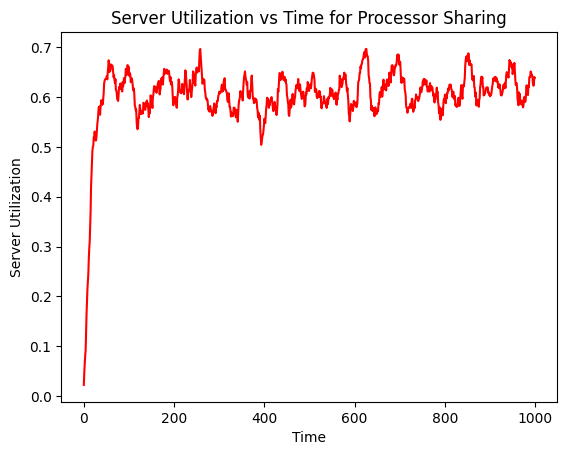
\includegraphics[scale=0.5]{fig_1.png}
     \caption{Processor sharing server utilisation}
\end{figure}


\begin{figure}[H]
     \centering
     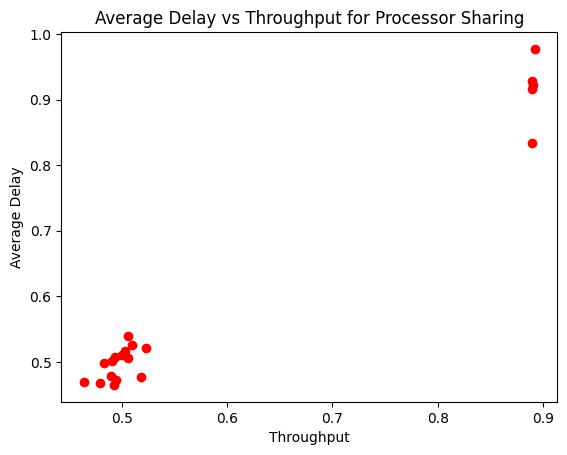
\includegraphics[scale=0.5]{fig_2.png}
     \caption{Average Delay vs Throughput}
\end{figure}

\subsection{Scheme 2: Water Filling or minimise the max queue}
The scheme is as follows: Let flow $i$ have $Qi(t)$ number of packets at time $t$. Serve the flows in such a way that at $t+1$, the gap $max_i Qi(t+1)-min_i Qi(t+1)$ is minimized. \\There is an iterative way of doing this, let's say my service capacity for this time slot is $S$. Then until S=0, I can go on decreasing S by 1 by serving 1 packet from the current maximum queue at every step. Since, at every step, I am making the greedy choice of minimising the gap $max_i Qi(t+1)-min_i Qi(t+1)$, then after all S capacity has been used, the current queues are the optimal queues and the packets served are optimal as per the water filling scheme.\\

Consider $S=11$, queue sizes: $Q = (7,3,2,1)$, then after this time slot, the queue sizes would be: $Q = (0,0,1,1)$.

\begin{itemize} 
\item Step 1: Queue 1 is max, keep serving it till it is max: $Q=(2,3,2,1)$ and S=6.
\item Step 2: Queue 2 is max:  $Q=(2,1,2,1)$ and S=4.
\item Step 3: Continue the same: $Q = (0,0,1,1)$ and S=0.
\end{itemize}
This is done in code as follows:

\begin{lstlisting}[language=Python]
#Scheme 2: Water filling or minimising the max queue
for t in range(T):
    #defining arrivals
    for i in range(K):
        if(arrival_bernoulli(probability_of_arrival[i])):
            arrival_times[i].append(t)
            queue_size[i] += 1
    #total service capacity
    S = service(N, K)
    S_copy = S

    #servicing
    #at each time slot, serve the flow with the maximum queue size
    while(S>0):
        #finding the flow with the maximum queue size
        max_queue = 0
        for j in range(K):
            if(queue_size[j] > max_queue):
                max_queue = queue_size[j]
                max_flow = j
        #serving the flow with the maximum queue size
        if(max_queue == 0):
            break
        service_times[max_flow].append(t)
        queue_size[max_flow] -= 1
        number_of_packets_served[max_flow][t] += 1
        S -= 1

    #server utilization
    if(S_copy == 0):
        server_utilization[t] = 0
    server_utilization[t] = (S_copy - S)/S_copy

    #updating average delay and probability of arrival for each flow
    for i in range(K):
        if(number_of_packets_served[i][t] > 0):
            #total packets served so far
            total = 0
            for j in range(t-1):
                total = total + number_of_packets_served[i][j]
            for j in range(number_of_packets_served[i][t]):
                average_delay[i] = average_delay_update(i, R, average_delay[i], t - arrival_times[i][total + j], total+j)
            probability_of_arrival[i] = arrival_general_update(i, probability_of_arrival[i], total, t, average_delay[i], R, arrival_times[i], service_times[i], 0.01)

#plotting moving average of server utilization
moving_average = [0 for i in range(T)]
for i in range(T):
    total = 0
    for j in range(20):
        if(i-j >= 0):
            total = total + server_utilization[i-j]
    moving_average[i] = total/20
plt.plot(moving_average, 'b')
plt.xlabel('Time')
plt.ylabel('Server Utilization')
plt.title('Server Utilization vs Time for Water Filling')
plt.show()

#throughput and average delay for each flow
throughput = [0 for i in range(K)]
for i in range(K):
    throughput[i] = len(service_times[i])/T

#plotting throughput and average delay for each flow
plt.plot(throughput, average_delay, 'bo')
plt.xlabel('Throughput')
plt.ylabel('Average Delay')
plt.title('Average Delay vs Throughput for Water Filling')
plt.show()

throughput_water_filling = throughput
average_delay_water_filling = average_delay
server_utilization_water_filling = server_utilization
moving_average_water_filling = moving_average

\end{lstlisting}

\begin{figure}[H]
     \centering
     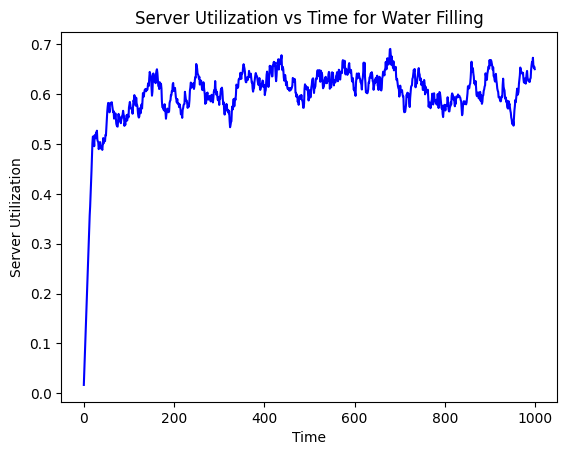
\includegraphics[scale=0.5]{fig_3.png}
     \caption{Water filling server utilisations}
\end{figure}

\begin{figure}[H]
     \centering
     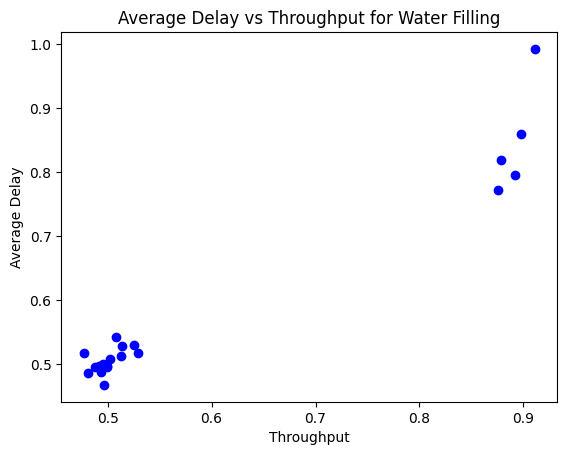
\includegraphics[scale=0.5]{fig_4.png}
     \caption{Average Delay vs Throughput}
\end{figure}

\subsection{Scheme 3: MaxWeight}
In this scheme, at every time step, we try to serve the maximum queue size first and then continue onto the smaller queues, if capacity is left. This is done in the following way, let's say at time step $t$, we have a service capacity $S$, we first find the maximum queue size and serve it entirely (or) as much as possible as per our capacity. If this queue is over, and we still have some capacity left, we serve the next maximum queue entirely (or) as much as possible and so on. \\\\
Consider $S=11$, queue sizes: $Q = (7,3,2,1)$, then after this time slot, the queue sizes would be: $Q = (0,0,1,1)$.

\begin{itemize}
\item Step 1: Serve the max queue. $Q = (0,3,2,1)$ and S=4.
\item Step 2: Serve the max queue. $Q = (0,0,2,1)$ and S=1.
\item Step 3: Serve the max queue (as much as possible). $Q = (0,0,1,1)$ and S=0.
\end{itemize}

This algorithm is executed in code as follows:


\begin{lstlisting}[language=Python]
#Scheme 3: MaxWeight
for t in range(T):
    #defining arrivals
    for i in range(K):
        if(arrival_bernoulli(probability_of_arrival[i])):
            arrival_times[i].append(t)
            queue_size[i] += 1
    #total service capacity
    S = service(N, K)
    S_copy = S

    #servicing
    #at each time slot, give all S slots to the flow with the maximum weight (queue size)
    while(S>0):
        #finding the flow with the maximum queue size
        max_queue = 0
        for j in range(K):
            if(queue_size[j] > max_queue):
                max_queue = queue_size[j]
                max_flow = j
        if(max_queue == 0):
            break
        for i in range(max_queue):
            if(S == 0):
                break
            service_times[max_flow].append(t)
            queue_size[max_flow] -= 1
            number_of_packets_served[max_flow][t] += 1
            S -= 1
    
    #server utilization
    if(S_copy == 0):
        server_utilization[t] = 0
    server_utilization[t] = (S_copy - S)/S_copy
    
    #updating average delay and probability of arrival for each flow
    for i in range(K):
        if(number_of_packets_served[i][t] > 0):
            #total packets served so far
            total = 0
            for j in range(t-1):
                total = total + number_of_packets_served[i][j]
            for j in range(number_of_packets_served[i][t]):
                average_delay[i] = average_delay_update(i, R, average_delay[i], t - arrival_times[i][total + j], total+j)
            probability_of_arrival[i] = arrival_general_update(i, probability_of_arrival[i], total, t, average_delay[i], R, arrival_times[i], service_times[i], 0.01)

#plotting moving average of server utilization
moving_average = [0 for i in range(T)]
for i in range(T):
    total = 0
    for j in range(20):
        if(i-j >= 0):
            total = total + server_utilization[i-j]
    moving_average[i] = total/20
plt.plot(moving_average, 'g')
plt.xlabel('Time')
plt.ylabel('Server Utilization')
plt.title('Server Utilization vs Time for MaxWeight')
plt.show()   

#throughput and average delay for each flow
throughput = [0 for i in range(K)]
for i in range(K):
    throughput[i] = len(service_times[i])/T

#plotting throughput and average delay for each flow
plt.plot(throughput, average_delay, 'go')
plt.xlabel('Throughput')
plt.ylabel('Average Delay')
plt.title('Average Delay vs Throughput for MaxWeight')
plt.show()

throughput_max_weight = throughput
average_delay_max_weight = average_delay
server_utilization_max_weight = server_utilization
moving_average_max_weight = moving_average

\end{lstlisting}

\begin{figure}[H]
     \centering
     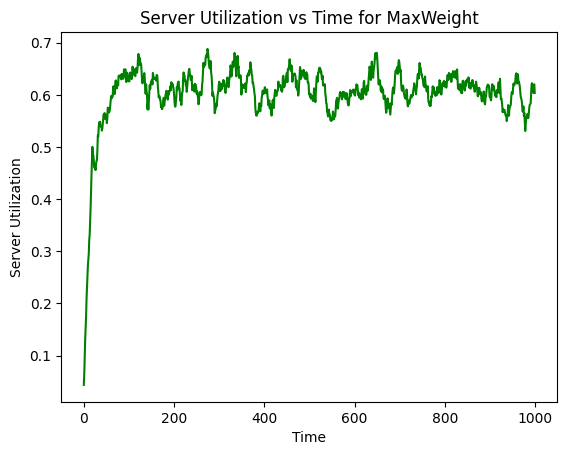
\includegraphics[scale=0.5]{fig_5.png}
     \caption{MaxWeight Server Utilisation}
\end{figure}

\begin{figure}[H]
     \centering
     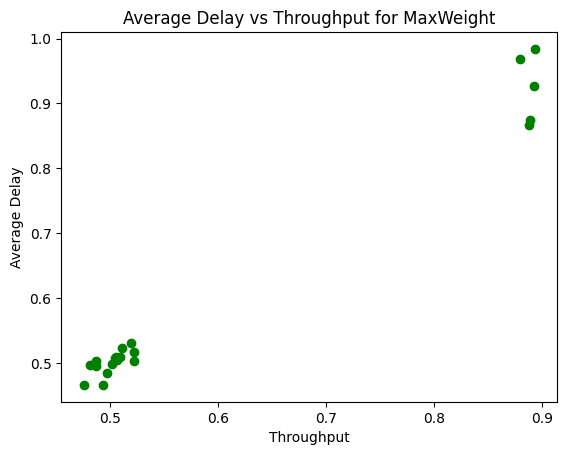
\includegraphics[scale=0.5]{fig_6.png}
     \caption{Average Delay vs Throughput}
\end{figure}

\subsection{Comparing the three Schemes}
Above, we have seen all the three schemes, the way they are executed, the algorithms and the simulation results. Now, we shall try to compare all these schemes and draw conclusions from our comparisons. 
Let us first plot the average delay vs throughputs for all the three schemes on the same plot.

\begin{figure}[H]
     \centering
     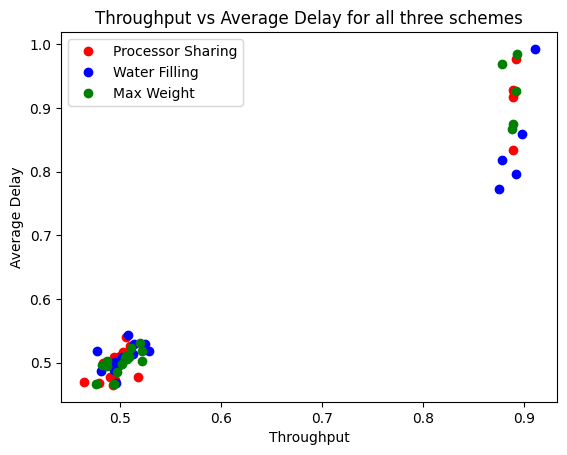
\includegraphics[scale=0.5]{fig_7.png}
     \caption{Average Delay vs Throughput for all three schemes}
\end{figure}

This does not give us any real distinctions between the three schemes in terms of average delay or throughput. \\
Let us take one particular flow, say flow 17 and try to observe the average delays and throughputs for that flow.\\
Consider the following codeblock:

\begin{lstlisting}[language=Python]
#Comparing throughput and average delay for all three schemes for a particular flow
pipe = 17
print("Throughput for flow", pipe, "for Processor Sharing Scheme:", throughput_processor_sharing[pipe-1])
print("Average Delay for flow", pipe, "for Processor Sharing Scheme:", average_delay_processor_sharing[pipe-1])
print("Throughput for flow", pipe, "for Water Filling Scheme:", throughput_water_filling[pipe-1])
print("Average Delay for flow", pipe, "for Water Filling Scheme:", average_delay_water_filling[pipe-1])
print("Throughput for flow", pipe, "for Max Weight Scheme:", throughput_max_weight[pipe-1])
print("Average Delay for flow", pipe, "for Max Weight Scheme:", average_delay_max_weight[pipe-1])

#Plotting throughput vs average delay for all three schemes for a particular flow
plt.plot(throughput_processor_sharing[pipe-1], average_delay_processor_sharing[pipe-1], 'ro', label = 'Processor Sharing')
plt.plot(throughput_water_filling[pipe-1], average_delay_water_filling[pipe-1], 'bo', label = 'Water Filling')
plt.plot(throughput_max_weight[pipe-1], average_delay_max_weight[pipe-1], 'go', label = 'Max Weight')
plt.xlabel('Throughput')
plt.ylabel('Average Delay')
plt.title('Throughput vs Average Delay for flow ' + str(pipe))
plt.legend()
plt.show()

\end{lstlisting}

The output is as follows:
\begin{figure}[H]
     \centering
     \includegraphics[scale=0.2]{fig_9.png}
     \caption{Output}
\end{figure}


\begin{figure}[H]
     \centering
     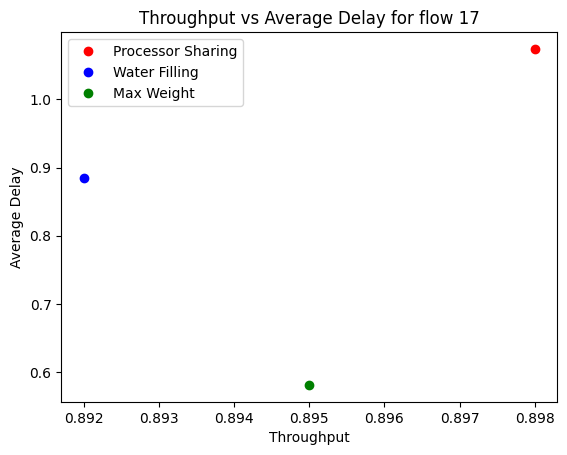
\includegraphics[scale=0.5]{fig_11.png}
     \caption{Throughput vs Average Delay for Flow 17}
\end{figure}

This shows us that the throughput is maximum for the Processor Sharing scheme, at the same time the average delay was minimum for the MaxWeight scheme. However, these results were not obtained constantly and hence no conclusions can be drawn between the choice of scheme and average delay and throughput.\\

Let us now try to compare the server utilisations for the three schemes.
For this, we plot the server utilisations versus time for all the three schemes on the same plot, and also print their time averages.

This was done using the following codeblock:
\begin{lstlisting}[language=Python]
#Plotting server utilizations of all three schemes on the same graph
plt.plot(moving_average_processor_sharing, 'r', label = 'Processor Sharing')
plt.plot(moving_average_water_filling, 'b', label = 'Water Filling')
plt.plot(moving_average_max_weight, 'g', label = 'Max Weight')
plt.xlabel('Time')
plt.ylabel('Server Utilization')
plt.title('Server Utilization vs Time for all three schemes')
plt.legend()
plt.show()
#comparing average server utilization for all three schemes in percentage
print("Average server utilization for Processor Sharing Scheme in percentage:", np.mean(server_utilization_processor_sharing)*100)
print("Average server utilization for Water Filling Scheme in percentage:", np.mean(server_utilization_water_filling)*100)
print("Average server utilization for Max Weight Scheme in percentage:", np.mean(server_utilization_max_weight)*100)

\end{lstlisting}


\begin{figure}[H]
     \centering
     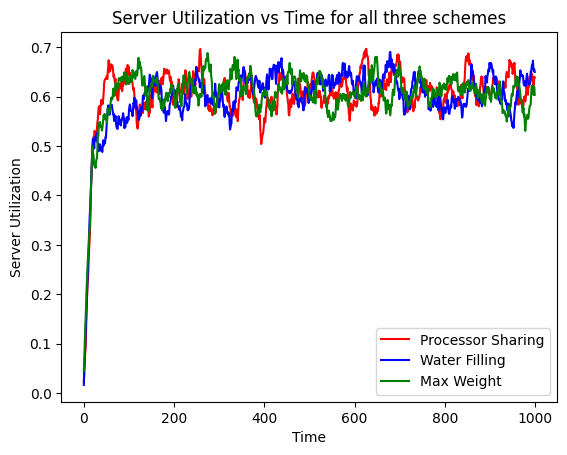
\includegraphics[scale=0.5]{fig_8.png}
     \caption{Output}
\end{figure}
\begin{figure}[H]
     \centering
     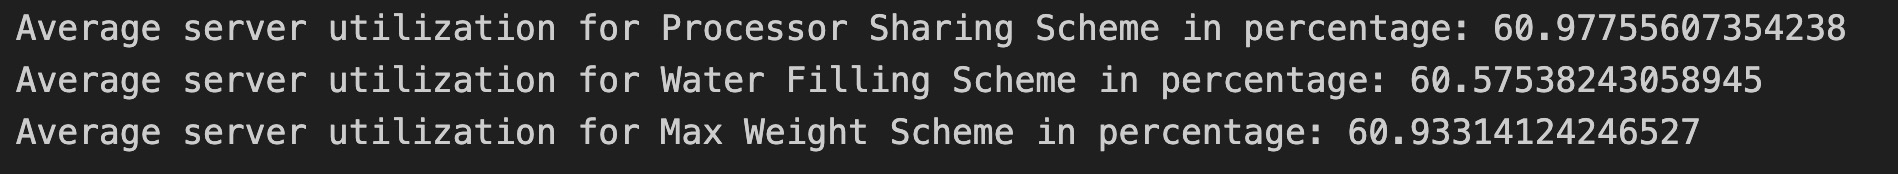
\includegraphics[scale=0.2]{fig_10.png}
     \caption{Output}
\end{figure}

\subsection{Server Utilisation versus arrival rate}
Let us now try to see the correlation between server utilisation and arrival rate for all the three schemes. 
Let us first try for $p$ very close to 0, say $p = 0.05$. Obtained results:

\begin{figure}[H]
     \centering
     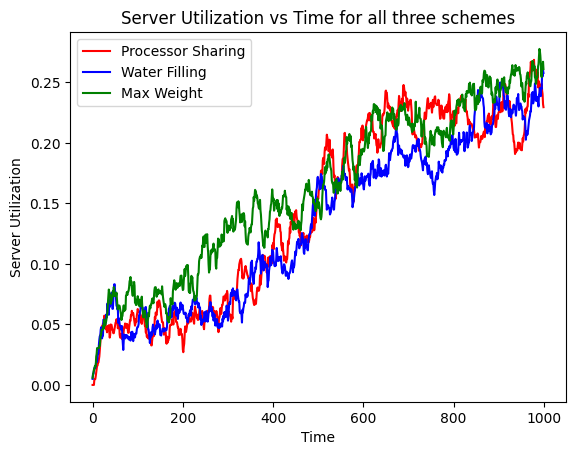
\includegraphics[scale=0.5]{su1.png}
     \caption{Server Utilisation for p=0.05}
\end{figure}

Clearly, for all three schemes, server utilisation seems to increase with time, this is because for all the $K-R$ flows, $p$ is TCP like and dynamically increases with time and thus server utilisation increases, since more packets come in with time. Average:

\begin{figure}[H]
     \centering
     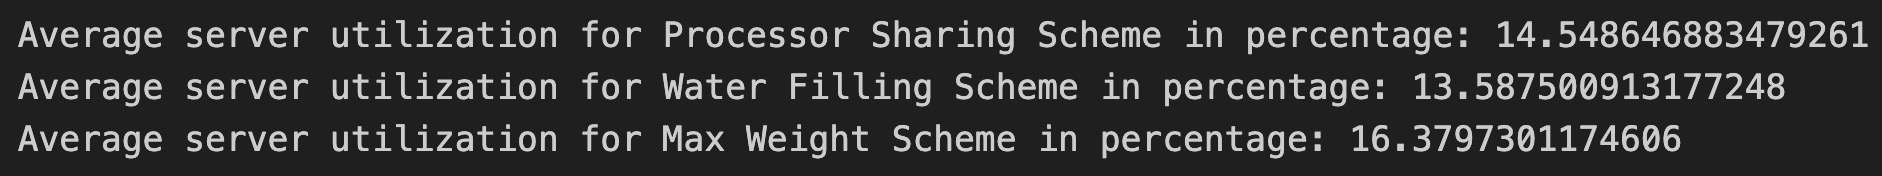
\includegraphics[scale=0.2]{su2.png}
     \caption{Output}
\end{figure}

Let us now simulate for a very high $p$ value, say $p=0.95$. Obtained results:
\begin{figure}[H]
     \centering
     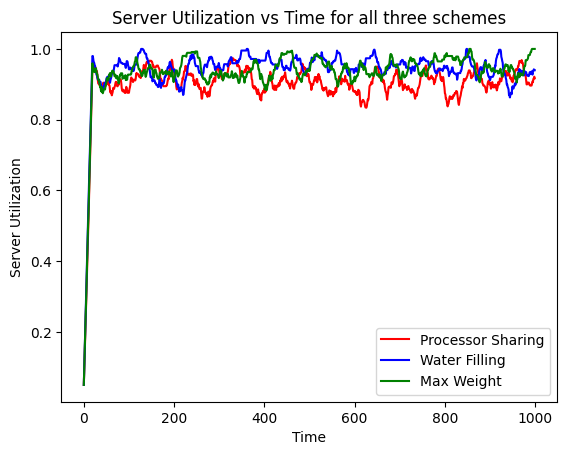
\includegraphics[scale=0.5]{su3.png}
     \caption{Server Utilisation for p=0.05}
\end{figure}

The server utilisations for all three schemes reach their highest values very quickly and thereby remain almost constant for the entire duration, since $p$ can decay to $0.9$ dynamically for the $K-R$ flows, even if it decays, there is not much change from $0.95$ to $0.90$ and that is why we don't see a great change in server utilisation.

\begin{figure}[H]
     \centering
     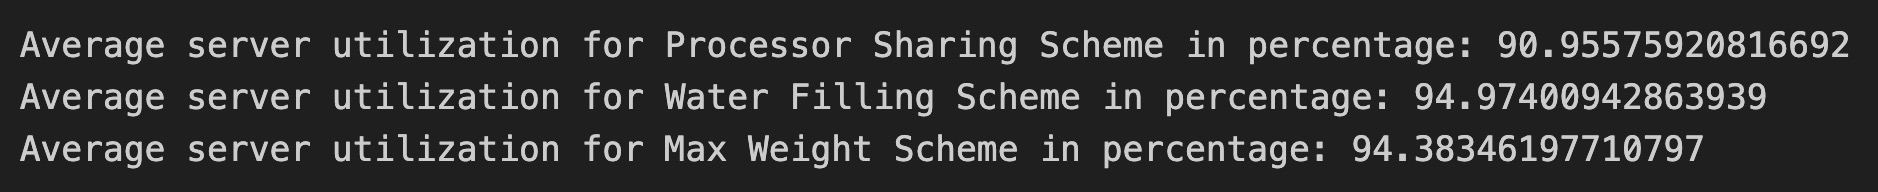
\includegraphics[scale=0.2]{su4.png}
     \caption{Output}
\end{figure}

\subsection{Changing (K,R)}
All the results up until now were for the $(K,R) = (20,15)$ pair, let us now try to simulate for $(K,R) = (5,1)$ and $(K,R) = (50,40)$ pairs, for $p=0.5$.

\subsubsection{(K,R) = (5,1)}
Taking $N=\lceil 1.1K \rceil=6$, we get:\\
Average Server Utilisations:
\begin{itemize}
\item Processor Sharing: 81.08\%
\item Water Filling: 81.32\%
\item MaxWeight: 81.30\%
\end{itemize}

Taking $N=\lceil 1.5K \rceil=8$, we get:\\
Average Server Utilisations:
\begin{itemize}
\item Processor Sharing: 81.85\%
\item Water Filling: 84.83\%
\item MaxWeight: 82.88\%
\end{itemize}

Taking $N=\lceil 3K \rceil=15$, we get:\\
Average Server Utilisations:
\begin{itemize}
\item Processor Sharing: 77.98\%
\item Water Filling: 83.12\%
\item MaxWeight: 82.90\%
\end{itemize}

\subsubsection{(K,R) = (50,40)}
Taking $N=\lceil 1.1K \rceil=55$, we get:\\
Average Server Utilisations:
\begin{itemize}
\item Processor Sharing: 58.08\%
\item Water Filling: 57.62\%
\item MaxWeight: 57.33\%
\end{itemize}

Taking $N=\lceil 1.5K \rceil=75$, we get:\\
Average Server Utilisations:
\begin{itemize}
\item Processor Sharing: 58.89\%
\item Water Filling: 58.23%
\item MaxWeight: 58.19%
\end{itemize}

Taking $N=\lceil 3K \rceil=150$, we get:\\
Average Server Utilisations:
\begin{itemize}
\item Processor Sharing: 58.73%
\item Water Filling: 58.22%
\item MaxWeight: 58.10%
\end{itemize}

Here, we clearly note that a if $\frac{R}{K}$ is higher, then server utilisation is low, this is because, these R flows do not dynamically update in a TCP like fashion and thus, lead to a lower average arrival rate and thus, lower server utilisations. Whereas, if $\frac{R}{K}$ is lower, then server utilisation is higher, because the $K-R$ flows dynamically update their arrival rates in order to maximise server utilisation for any scheme. 








\section{Finite Buffer Size}
In the case of the finite buffer, we might have some packets which are "dropped", i.e any packet which is arriving to a full buffer will not be entertained, and will be dropped, thus will have to be sent again by the sender. \\

We simulate the case of finite buffers for all three schemes in a similar way with just some slight modifications to the code to handle the buffer.

The function \texttt{arrival{\_}general{\_}update} is modified as following to take into account dropped packets. This is because though a dropped packet will not contribute to the update of $T_n^{(i)}$, but it will contribute to the number of un-served packets that arrived on or before $t-\left\lceil 1.2 T_{n(t)}^{(i)}\right\rceil$.

\begin{lstlisting}[language=Python]
def arrival_general_update(i, p, n, t, T, R, arrival_times, service_times, delta, dropped_times):
    #This is the update equation for the probability of arrival
    #p is the previous probability of arrival
    #n is the number of packets served so far for this flow
    #T is the average delay for this flow
    #arrival_times is the list of arrival times for this flow
    #service_times is the list of service times for this flow
    #This function returns the new probability of arrival
    if n == 0:
        return p
    elif i<R:
        return p
    elif len(arrival_times) > len(service_times):
        if(arrival_times[len(service_times)] <= t - np.ceil(1.2*T)):
            return 2*p/3
    elif len(dropped_times) > 0:
        if dropped_times[0] <= t - np.ceil(1.2*T):
            #remove first element of dropped_times
            dropped_times= dropped_times.pop(0) #count one dropped packet only once
            return 2*p/3
    #for the 2nd case,
    #the first packet served in this time slot should have arrived 
    #at most 1.2*T time slots ago
    else:
        for i in range(len(service_times)):
            if service_times[i] == t:
                if arrival_times[i] > t - np.ceil(1.2*T): #checking if the served packet arrived in the last 1.2*T time slots
                    return min(0.9, p+delta)
                else:
                    break
    return p
\end{lstlisting}

The algorithms remain the same for all three schemes, which just a slight change in which input arrivals are handled. The change is:

\begin{lstlisting}[language=Python]
#defining arrivals
    for i in range(K):
        if(arrival_bernoulli(probability_of_arrival[i])):
            if(queue_size[i] < q_max):
                queue_size[i] += 1 #increment queue size if buffer is not full
                arrival_times[i].append(t)
            else:
                dropped_packets[i] += 1 #increment dropped packets if buffer is full
                dropped_times[i].append(t)
\end{lstlisting}

This makes sure that only those packets which can still fit in the buffer are counted in \texttt{arrival{\_}times} and those which are dropped are counted in \texttt{dropped{\_}times} and increment \texttt{dropped{\_}packets}. \\

We simulate for buffer sizes $\alpha \frac{Kp^2}{1-p}$ for $\alpha = 1.2, 1.5, 3$, for all the three schemes and try to observe the results.

Running the code for $\alpha = 1.2$and observing throughput and delay for flow 17, we get:


\begin{figure}[H]
     \centering
     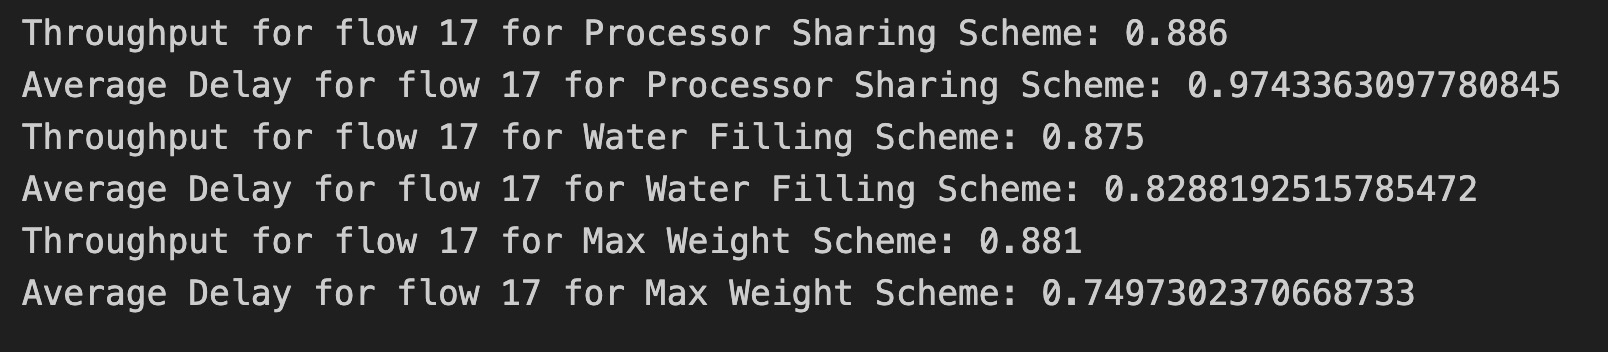
\includegraphics[scale=0.2]{fig_a.png}
     \caption{Output}
\end{figure}

Not a very significant difference as compared to the infinite buffer case. Let us try to observe the server utilisations, we get:

\begin{figure}[H]
     \centering
     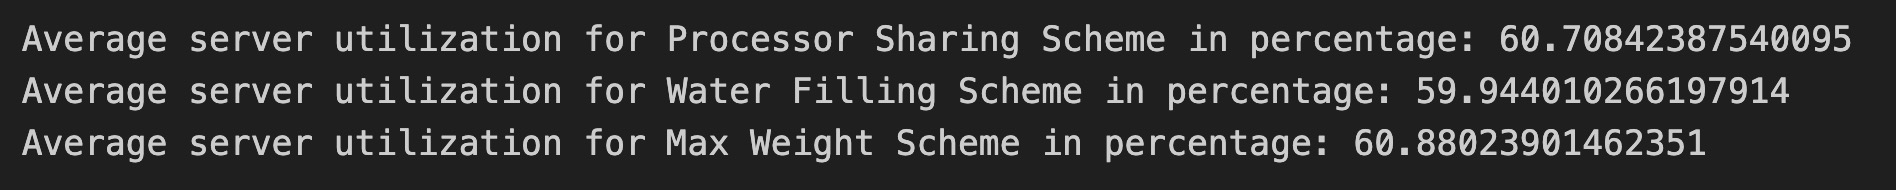
\includegraphics[scale=0.2]{fig_b.png}
     \caption{Output}
\end{figure}

Yet again, these values do not sway too much as compared to the values for the infinite buffer case. Anyways, let's try to observe how many packets are dropped for each flow, maybe that can give us a hint about what is happening.

Printing the number of dropped packets for each flow, we get:
\begin{figure}[H]
     \centering
     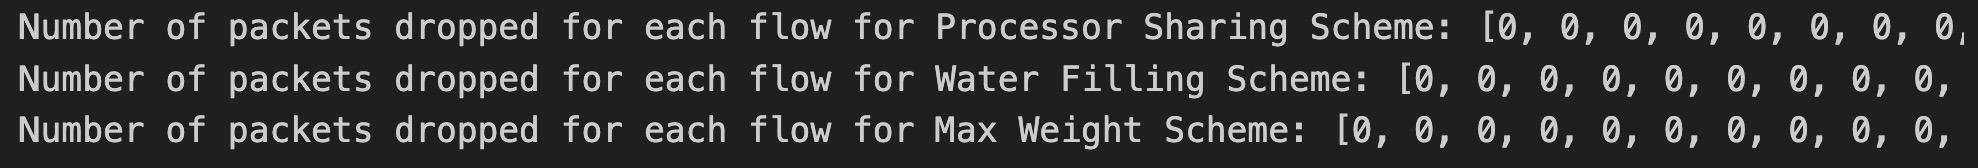
\includegraphics[scale=0.2]{fig_c.png}
     \caption{Output}
\end{figure}

We get only 0's as the number of packets dropped for any flow, so something interesting is happening here, no packets are being dropped i.e the finite buffer case is as good as the infinite buffer case for $\alpha = 1.2$, if the buffer size corresponding to $\alpha = 1.2$ is able to handle all packets, then obviously $\alpha = 1.5, 3$ can handle all packets\\

An intuitive reason of why this happens is the following, the server has a $Binomial(N,K/N)$ distribution, which means that the expected capacity at any time slot is $N*K/N = K$, since the expected number of arriving packets is only $p_{avg}*K$, the server is efficiently able to handle all these arrivals and thus the queue sizes never get even remotely big, which we had seen in the infinite buffer case, all our average queue sizes were always less than 1.\\

Thinking on parallel lines, what if we increase p to 0.99, i.e as close to 1 as possible, on simulating this case, we observe that the number of packets dropped for this case is also 0 for all flows, thus indicating that increasing p did not cause packets to drop for a fixed $\alpha$.

Similarly, decreasing $K$ did not cause packets to drop either, and thus we can conclude that among the three $\alpha = 1.2, 1.5, 3$, $\alpha=1.2$ is sufficient enough to handle this system.


\section{Conclusion}
We have simulated the given caricature TCP model and have studied three scheduling algorithms namely processor sharing, water filling and MaxWeight scheduling, we noticed that for small arrival rates the server utilisation tends to increase with time as the arrival rates dynamically increase in a TCP like fashion, whereas for higher arrival rates, server utilisation is more or less constant.\\


An interesting point to note was that server utilisation was higher for lower values of $\frac{R}{K}$, this is because more number of flows were dynamic since $K-R$ was larger. Also, server utilisation is higher for higher arrival rates. It would be an interesting topic of research to study how the interplay of static and dynamic flows, along with arrival rates affects the server utilisation, while at the same time ensuring that queue lengths do not get large enough that a small finite buffer is unable to handle it, and packets start dropping. The interplay of all these factors with each other should be an interesting direction to research in. \\Another interesting problem could be with respect to buffer sizes, in the simulations we noticed that we were able to get $0$ packets dropped for the given buffer sizes, an interesting problem could be to study about how small our buffer could be so that even after dropping a few packets, we're able to maximise server utilisation and throughput. \\
The code can be found here: \href{https://drive.google.com/drive/folders/1NdwyRu0YszZP-SYvFp2CQcfdz0ehORMg?usp=sharing}{Code}\\

\end{document}



 